% Compile with XeLaTeX, TeXLive 2013 or more recent
\documentclass{beamer}

% Base packages
\usepackage{fontspec}
\usepackage{xunicode}
\usepackage{xltxtra}

\usepackage{amsfonts}
\usepackage{amsmath}
\usepackage{longtable}
\usepackage{csquotes}
\usepackage{standalone}
\usepackage{bytefield}

% Setup fonts
\newfontfamily\russianfont{CMU Serif}
\setromanfont{CMU Serif}
\setsansfont{CMU Sans Serif}
\setmonofont{CMU Typewriter Text}

% Setup Russian hyphenation. NOTE: this declaration *must* come after fontspec's font declarations,
% or a mysterious (but harmless in other respects) error "Improper `at' size (0.0pt), replaced by 10pt." would appear.
\usepackage{polyglossia}
\defaultfontfeatures{Scale=MatchLowercase, Mapping=tex-text}

\setdefaultlanguage[spelling=modern]{russian} % for polyglossia
\setotherlanguage{english} % for polyglossia

% Vector drawings
\usepackage{tikz}
% \usetikzlibrary{shapes, calc, arrows, fit, positioning, decorations, patterns, decorations.pathreplacing, chains, snakes}
\usetikzlibrary{shapes, calc, arrows, decorations.markings, decorations.pathmorphing, decorations, patterns, chains, snakes, backgrounds, positioning, fit, petri}
\usepackage[siunitx]{circuitikz}

% Be able to insert hyperlinks
\usepackage{hyperref}
\hypersetup{colorlinks=true, linkcolor=black, filecolor=black, citecolor=black, urlcolor=blue , pdfauthor=Grigory Rechistov <grigory.rechistov@phystech.edu>, pdftitle=Курс «Программное моделирование вычислительных систем»}
% \usepackage{url}

% Misc optional packages
\usepackage{underscore}
\usepackage{amsthm}

% A new command to mark not done places
\newcommand{\todo}[1][Напиши меня]{{\color{red}TODO\ #1}}
\newcommand{\abbr}{\textit{англ.}\ }

\title{Моделирование архитектурного состояния}
\subtitle{Курс «Программное моделирование вычислительных систем»}
\subject{Курс «Программное моделирование вычислительных систем»}

\author[]{Григорий Речистов \\ \small{\href{mailto:grigory.rechistov@phystech.edu}{grigory.rechistov@phystech.edu}}}
\date{\today}
\pgfdeclareimage[height=0.5cm]{ilab-logo}{../ilab-noletters.png}
\logo{\pgfuseimage{ilab-logo}}

\typeout{Copyright 2015 Grigory Rechistov}

\usetheme{Berlin}
\setbeamertemplate{navigation symbols}{}%remove navigation symbols

\begin{document}

\begin{frame}
    \maketitle
\end{frame}

\begin{frame}
    \tableofcontents
\end{frame}

\section*{Обзор}

\begin{frame}{На прошлой лекции}
Интерпретаторы — простой метод создания моделей процессоров

\end{frame}

\begin{frame}{Вопросы}
\begin{itemize}
\item Чем декодирование отличается от дизассемблирования? \pause
\item Чем прерывание отличается от исключения? \pause
\item Может ли сцепленный интерпретатор быть кэширующим?
\end{itemize}

\end{frame}

% «»

\begin{frame}{Платформа}
\centering
\vfill
\input{./../../simbook/metoda/drawings/full-platform}
\vfill

\end{frame}

\section{Регистровый файл}

\begin{frame}{Регистровый файл}
\centering
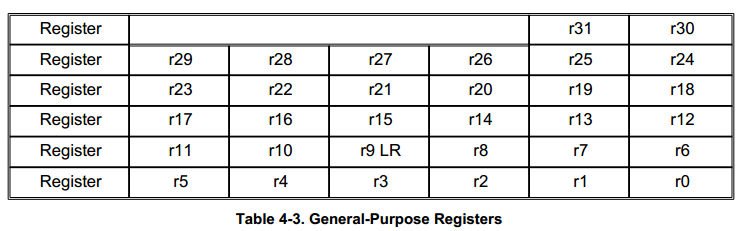
\includegraphics[width=0.8\textwidth]{or1k-gprs}

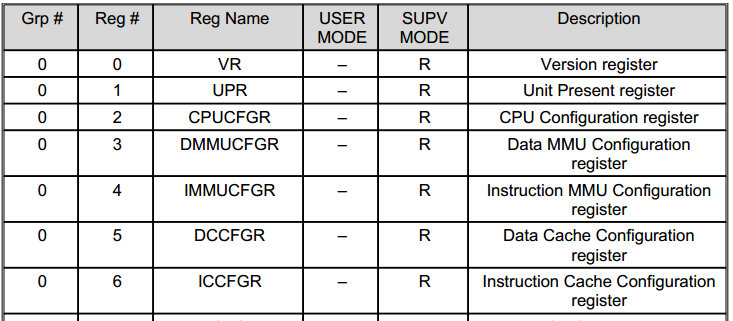
\includegraphics[width=0.8\textwidth]{or1k-sprs}

\tiny{OpenCores. OpenRISC 1000 Architecture Manual rev 1.0}
\end{frame}

\begin{frame}[fragile]{С-структура}
\begin{verbatim}
#include <stdint.h>
#define NO_GPRS 32
#define NO_SPRS 1024
#define REG_VR 0
#define REG_UPR 1
/* ... */
typedef struct cpu {
    uint32_t pc;
    uint32_t gprs[NO_GPRS];
    uint32_t sprs[NO_SPRS];
} cpu_t;
\end{verbatim}

\end{frame}

\begin{frame}{Хозяйские регистры}
\begin{itemize}
\item Доступ к структуре в памяти медленный
\item Доступ к хозяйским регистрам быстрее
\item Разместим гостевые регистры на хозяйских!
\item \texttt{register cpu_t* cpu __asm__("rbp");}
\end{itemize}
\end{frame}

\begin{frame}[fragile]{Хозяйские регистры}
\begin{itemize}
\item Все гостевые регистры могут не поместиться
\item Есть смысл размещать только самые часто используемые
\item Потеря переносимости кода
\item Специализация регистров: PC, SP, FP[0-7]
\item Мы мешаем работе компилятора: давление на регистры
\end{itemize}
\end{frame}

\section{Ленивое вычисление состояния}
\begin{frame}{Ленивое вычисление состояния}
\begin{itemize}
\item Вообще не вычислять состояние, пока оно не понадобится!
\item Пример: IA-32 \texttt{EFLAGS}
\item $flags = f(a, b, op)$ для последней инструкции, влияющей на флаги
\end{itemize}

\centering
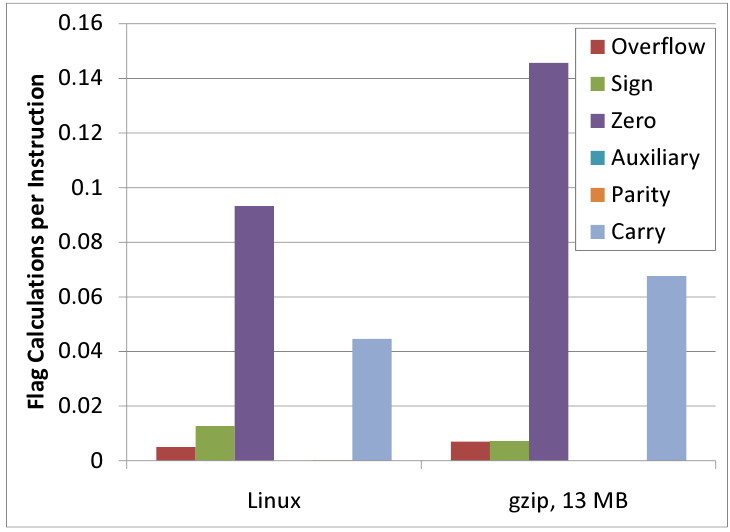
\includegraphics[width=0.5\textwidth]{lazy-eflags}

\tiny{Yair Lifshitz et al. Zsim: A Fast Architectural Simulator for ISA Design-Space Exploration}
\end{frame}

\section{Большие массивы}

\begin{frame}[fragile]{Доступ к ОЗУ и большим массивам}
Просто выделить на куче!
\begin{verbatim}
uint8_t *buf = (uint8_t *)calloc(BUF_SIZE, 1);

/* read */
uint8_t val = buf[offset];

/* write */
buf[offset] = val;
\end{verbatim}
\pause
Что же делать, если, BUF_SIZE $\sim 2^{53}$, а хозяйской памяти в наличии $2^{32}$?
\end{frame}

\begin{frame}[fragile]{Ленивое выделение памяти}
Для непрерывного дипазона адресов хранилище выделяется по мере необходимости кусками фиксированного размера (страницами).

\begin{verbatim}
page = addr & PAGE_MASK;
hptr = lookup_hptr(page);
if (!hptr)
    hptr = allocate_hptr(page);
assert(hptr);
haddr = hptr + (addr & PAGE_OFFSET);
\end{verbatim}
При недостатке хозяйской памяти «старые» страницы выгружаются на диск.
\end{frame}

\begin{frame}[fragile]{Звучит знакомо?}
\begin{itemize}
\item Это же виртуальная память!
\item POSIX-системы предоставляют механизм mmap()
\end{itemize}

\begin{verbatim}
void *mmap(void *addr, 
    size_t len, int prot, int flags,
    int fildes, off_t off); 
\end{verbatim}

\centering

\begin{tikzpicture}[>=latex, font=\small, node distance=0mm, inner xsep=0pt, text width = 10mm, every node/.style=draw]

\begin{scope}[start chain]
    \node [on chain] (vp0) {};
    \node [on chain] {};
    \node [fill=black!10, on chain] (vp2) {};
    \node [fill=black!10, on chain] (vp3) {};
    \node [on chain] {};
    \node [on chain] {};
    \node [on chain] {};    
    \node [fill=black!10, on chain] (vp4) {};    
    \node [fill=black!10, on chain] (vp1) {};    
    \node [on chain] {};    
    \node [fill=black!10, on chain] (vp5) {};    
\end{scope}

\begin{scope}[start chain]
    \node [on chain, below=1cm of vp0] (pp1) {} ;
    \node [on chain] (pp2) {};
    \node [on chain] (pp3) {};
    \node [on chain] (pp4) {};

\end{scope}
    \node [right=2cm of pp4] (dp1) {};    

\draw[->] (vp1.south) -- (pp1.north);
\draw[->] (vp2.south) -- (pp2.north);
\draw[->] (vp3.south) -- (pp3.north);
\draw[->] (vp4.south) -- (pp4.north);
\draw[->] (vp5.south) -- (dp1.north);
    
\node[draw=none, above=0.1cm of vp0.east, text width=4cm, xshift=1cm] {Выделенный блок};
\node[draw=none, below=0.1cm of pp1.east, text width=4cm, xshift=1cm] {Физические страницы};
\node[draw=none, below=0.1cm of dp1.east, text width=4cm, xshift=1cm] {Дисковый своп};


\end{tikzpicture}

\end{frame}

\section{Регистры, поля, банки}

\begin{frame}[fragile]{Два способа взаимодействия с регистрами устройств}
PIO — programmable I/O, выделенные инструкции для общения с периферией (IA-32, IBM s390, PDP-8)

\begin{verbatim}
IN EAX, DX
OUT DX, EAX
\end{verbatim}
\pause

MMIO — memory mapped I/O, унифицированный подход к доступу к ОЗУ и устройствам (IA-32, ARM, PDP-11)

\begin{verbatim}
MOV [mem], reg
MOV reg, [mem]
\end{verbatim}

\end{frame}

\begin{frame}{Операции над регистрами}
\begin{itemize}
\item read, write, fetch, prefetch
\item Регистры-хранилище и регистры с побочными эффектами
\item Примеры регистров с side-effects: time stamp (RW), command (W), status (R), version (RO)
\item inquiry — «призрачное» обращение (без эффектов)
\item reset
\end{itemize}

\end{frame}

\begin{frame}[fragile]{Операции над регистрами}
\begin{verbatim}
template <class rtype> class IRegister {
  virtual Exception Read(rtype& retval) = 0;
  virtual Exception Fetch(rtype& retval) = 0;
  virtual Exception Prefetch(rtype& retval) = 0;
  virtual Exception Write(const rtype& newval) = 0;
  virtual bool InquiryRead(rtype& retval) = 0;
  virtual bool InquiryWrite(const rtype& newval) = 0;
  virtual void Reset() = 0;
}
\end{verbatim}
\end{frame}

\begin{frame}[fragile]{Битовые поля}

\begin{bytefield}[bitwidth=0.8em, endianness=big]{32}
\bitheader{31,19,18,17,16,15,13,12,11,8,7,0} \\
\bitbox{13}{}&\bitbox{2}{\tiny{mode}} & \bitbox{1}{\rotatebox{90}{\tiny{mask}}} & \bitbox{3}{} & \bitbox{1}{\rotatebox{90}{\tiny{status}}} & \bitbox{4}{} & \bitbox{8}{vector} \\
\end{bytefield}

\tiny{APIC LVT Timer. Intel® 64 and IA-32 Architectures Software Developer’s Manual}

\normalsize
\begin{itemize}
\item Настоящие базовые единицы спецификаций и моделирования
\item Могут иметь совершенно различные свойства внутри регистра
\end{itemize}

\end{frame}

\begin{frame}[fragile]{Банк регистров}
Группа регистров устройства, находящиеся в одной области
\vfill
\centering

\begin{tikzpicture}[font=\small, >=latex]

\node[text height=5cm, text width=1cm, draw]  (physspace) {

};

\node[right=of physspace] (bank) {
\begin{bytefield}[bitwidth=.5em, endianness=big]{32}
\bitheader{31, 0}\\
\wordbox{1}{reg_base}\\
\wordbox{1}{reg_offset}\\
\bitbox{25}{reg_cmd_in} & \bitbox{7}{rsvd}\\
\wordbox{2}{reg_data_out}\\
\end{bytefield}
};

\draw (physspace.10) -- ([yshift=-0.25cm]bank.north west);
\draw (physspace.350) -- ([yshift=0.5cm]bank.south west);

\node[left=0cm of physspace.north west] {\texttt{0x0}};
\node[left=0cm of physspace.south west] {\texttt{0xffff}};

\end{tikzpicture}

\end{frame}
\begin{frame}{Карты памяти}
\input{./../../simbook/metoda/drawings/memmap}
% \begin{itemize}
% \item 
% \item 
% \end{itemize}
\end{frame}

\begin{frame}{Пример: devmgmt.msc}
\centering
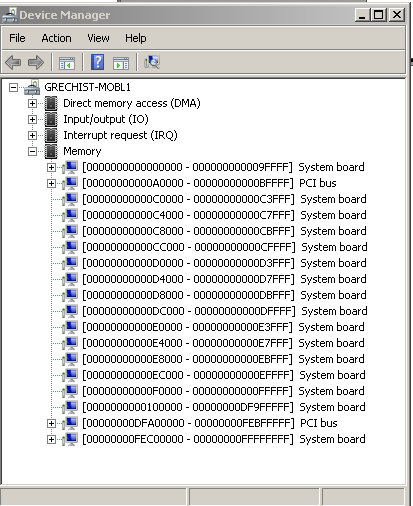
\includegraphics[width=0.6\textwidth]{devicemanager}
\end{frame}

\section{Прерывания}

\begin{frame}{Прерывания}
\begin{centering}
\input{./../../simbook/metoda/drawings/interrupt-line}
\end{centering}

\begin{itemize}
\item Как моделировать отдельное прерывание — очень просто:\\
\texttt{take_interrupt(dev_t *dev);}
\item Когда моделировать — вопрос сложнее, тема отдельной лекции
\end{itemize}

\end{frame}

\begin{frame}{Преобразование адресов}
\begin{itemize}
\item v2p
\item p2h
\item v2p + p2h =  v2h
% \item softTLB
\end{itemize}
\end{frame}

\section{Endianness}

\begin{frame}{Порядок байт при доступах}

\begin{columns}[onlytextwidth]
\begin{column}{0.5\textwidth}
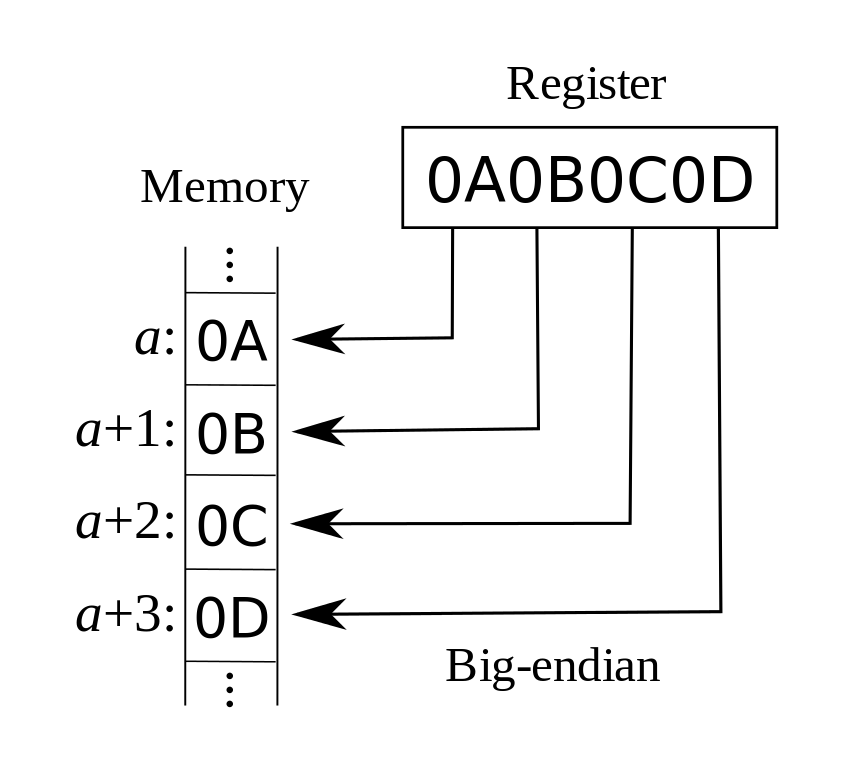
\includegraphics[width=\textwidth]{./be}
\end{column}

\begin{column}{0.5\textwidth}
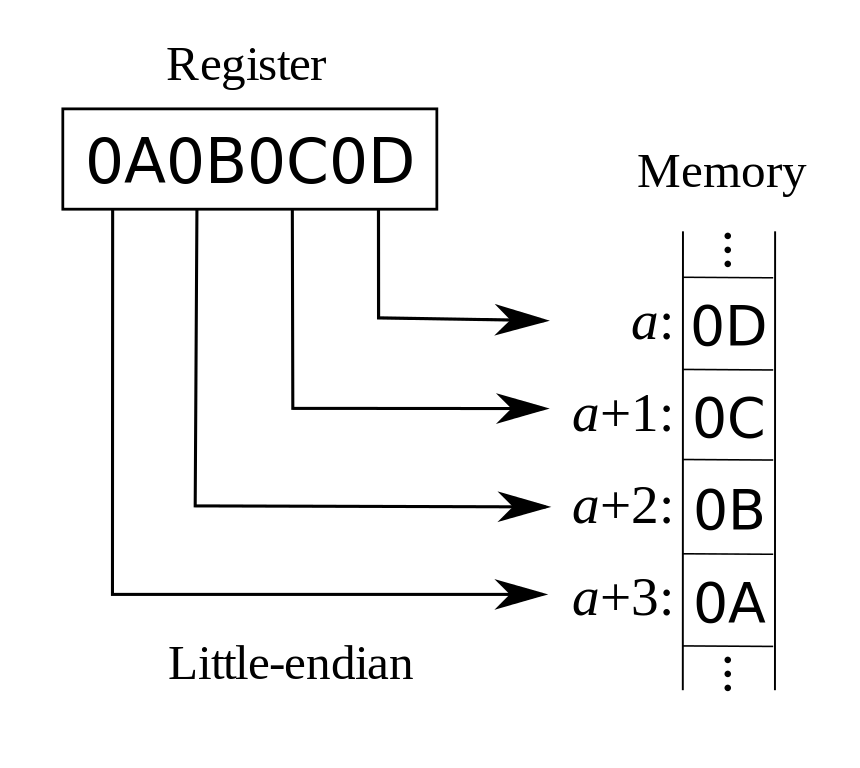
\includegraphics[width=\textwidth]{./le}
\end{column}
\end{columns}

% \begin{itemize}
    % \item Порядок от младшего к старшему (\abbr little-endian);
    % \item Порядок от старшего к младшему (\abbr big-endian);
% \end{itemize}

    % \item Смешанный порядок (\abbr middle-endian).


\end{frame}

\begin{frame}{Бит, байт, слово}
\begin{itemize}
\item Бит — кол-во информации, уменьшающее неопределённость в два раза\pause
\item Байт \pause — минимальная адресуемая (в данной архитектуре) единица хранения
информации \pause
\item Октет \pause — восемь бит \pause
\item Машинное слово \pause — максимальный объём информации, который ЦПУ может обработать единовременно
\end{itemize}

\pause
Intel: word — 16 бит, dword — 32 бит, qword — 64 бит.
\end{frame}



\section*{Литература}

\begin{frame}[allowframebreaks]{Литература}
\begin{thebibliography}{99}
    \bibitem{bochsunderhood} Stanislav Shwartsman, Darek Mihoka. How Bochs Works Under the Hood. 2nd edition.
    \url{http://bochs.sourceforge.net/How the Bochs works under the hood 2nd edition.pdf}
    
    \bibitem{bic} M. Domeika, M. Loenko, P. Ozhdikhin, E. Brevnov.  Bi-Endian Compiler: A Robust and High Performance Approach for Migrating Byte Order Sensitive Applications.
    \url{http://world-comp.org/p2011/ESA2902.pdf}
\end{thebibliography}
\end{frame}

\section*{Конец}
% The final "thank you" frame 

\begin{frame}{На следующей лекции}
\begin{itemize}
\item Делаем симулятор, работающий быстрее, чем интерпретатор
\item Двоичная трансляция
% \item Двоичная инструментация
\end{itemize}
\end{frame}

\begin{frame}

{\huge{Спасибо за внимание!}\par}

\vfill

Слайды и материалы курса доступны по адресу \url{http://is.gd/ivuboc} % http://atakua.doesntexist.org/wordpress/simulation-course-russian/

\vfill

\tiny{\textit{Замечание}: все торговые марки и логотипы, использованные в данном материале, являются собственностью их владельцев. Представленная здесь точка зрения отражает личное мнение автора, не выступающего от лица какой-либо организации.}

\end{frame}

\end{document}
